\chapter{Fast Pauli Element manipulation}
\label{appendix:FPPM}

Most of the Quantum processor using spin dynamics, so that the Pauli matrices and 
$n$-folded Pauli strings are major elements to analysis and to manipulation the system.
Common method to implement Pauli algebra is a matrix representation, for $l= 0, 1, 2, 3$.

\begin{equation*}
    \sigma_l \in \left\{ \begin{bmatrix} 1& 0 \\ 0 &1\end{bmatrix}, 
    \begin{bmatrix} 0& 1 \\ 1 &0\end{bmatrix},
    \begin{bmatrix} 0& -i \\ i &0\end{bmatrix},
    \begin{bmatrix} 1& 0 \\ 0 &-1\end{bmatrix} \right\}
\end{equation*}

Pauli elements of $n$ number of particle system are easily achieved by tensor product of the 
Pauli elements of single particle system. For $n$ number of $1/2$ spin particles, there are $4^n$ number of Pauli elements.

\begin{equation*}
    P^{(n)} = \otimes_{l=0}^{4^n} \sigma_{a_l}
\end{equation*}

where, $a_l = 0, 1, 2, 3$.
Since, tensor product is well established in matrix space as kronecker product,
we can manipulate and analysis the Pauli elements with matrix operations.
Mathematically, there is no huddle and any ambiguous to deal the elements in matrix form.
We can implement Pauli algebra in any number of particle system.

\begin{exercise}(Matrix representation of Pauli algebra)

    Show that the matrix representation of the above Pauli elements satisfy the next equations,
    For $i,j,k,l \in \{0, 1, 2, 3\}$,

    \begin{equation*}
        [\sigma_j, \sigma_k] = 2 i \epsilon_{jkl} \sigma_l
    \end{equation*}
    and
    \begin{equation*}
        \sigma_j \cdot \sigma_k = \delta_{jk} I + i  \epsilon_{jkl} \sigma_l
    \end{equation*}
\end{exercise}

\begin{exercise}(Orthonormality of $n$-fold Pauli elements)

    Using Hilbert Schmidt inner product and norm, show that the $n$-folded Pauli elements are form a complete basis of
    $M_{2^n}(\mathbb{C})$.
\end{exercise}

The problem arise in computational aspect. 
Matrix operation is proportional to the dimension of Hilbert space, however, the dimension grows exponentially, $O(2^n)$,
by the number of particle, $n$. When we want to calculate two Pauli elements we need $O(2^n)$ operations.
In addition, decomposing given Hamiltonian, constructing a Pauli element matrix are also growth exponentially.


\begin{align*}
    P_k = P_i P_j\\
    H = \sum_j \lambda_j P_j^{(n)} \\
    H \rightarrow_{decompose} \sum_j \lambda_j P_j^{(n)}\\
    H \leftarrow_{compose} \sum_j \lambda_j P_j^{(n)}
\end{align*}

\subsection*{Complexity of Matrix representation}

Assume that the multiplication and addition as same.

\begin{exercise}(Algebra complexity)

    For $n$-particle system, what is a time complexity to calculate $P_i P_j$ in matrix form?
\end{exercise}

In addition, if a Pauli element is given, can you directly determine what Pauli element in the Hilbert space?
Matrix elements gave you enough information to identify what element was it. 
However, It is hard to map the matrix to corresponding Pauli element.

\begin{exercise}(Decomposition)

    The standard process of Hamiltonian decomposition is using an inner product of Hamiltonian and Pauli elements,
    \begin{equation*}
        \lambda_j = \langle H | P_j^{(n)} \rangle_{HS} = \frac{1}{2^n} \tr(H^\dagger P_j^{(n)})
    \end{equation*}
    In $n$-particle system, what is a time complexity of single $\lambda_j = \langle H | P_j^{(n)} \rangle$ operation?
\end{exercise}

Let the answer of the above question as $f(n)$, then, since there are $4^n$ number of Pauli terms, 
the total complexity to decompose the Hamiltonian into Pauli terms becomes $O(f(n) 4^n)$.

\begin{exercise}(Composition)

    What is a time complexity to make a tensor product of two $n \times n$ and $m \times m$ dimension matrix?
    $n$ fold Pauli element is constructed by $n$ number of tensor product of $2 \times 2$ matrix.
    Calculate a time complexity to make a matrix form of single $n$-fold Pauli element by tensor product.
\end{exercise}

In the composition, we know the number of Pauli terms in the Hamiltonian.
Let the number as $k\in \{1, 4^n\}$. Then the total complexity is $O(k g(n))$. 
Therefore, the time complexity to make a matrix form of the given polynomial becomes at least $O(g(n))$, and 
maximally it becomes $O(4^n g(n))$. $g(n)$ would be an exponential value if you calculated well $g(n) \approx 8^n$. 

\section{Symplectic code representation}

Matrix representation is intuitive and easy to calculate, however, its computational complexity is poor.
In geometrical approach, researchers found that Pauli elements have a special property, \textit{symplectic}.
This interpretation gave us more convenience representation, \textit{symplectic representation}.

\begin{equation} 
    \label{eq:symplectic_pauli}
    P_j = (i)^f \hat{X}(a) \hat{Z}(b)
\end{equation}

Most of the quantum computing frameworks adopt symplectic code to manipulate the Pauli element efficiently.
There are requires mathematical backgrounds to understand the word symplectic and application in here
\footnote{Lie algebra, Clifford group and Differential geometry are required.}.
However, let us derive the result only with matrix and $\mathbb{Z}_2$ knowledges. 
If you are familiar with computational thinking, $\mathbb{Z}_2$ is just a classic bit manipulation.

$\sigma_0 = I, \sigma_1 = X, \sigma_2 = Y, \sigma_3 = Z$

\begin{example}(Symplectic representation in $n=1, 2$ Cases)

    $Y = -i XZ$
\end{example}
% Qskit, Pennylane, QuEra, PauliArray.




%-------------------
\subsection{Summary}

We can represent any Pauli elements

There are many references to deal the symplectic code, you can refer the code and documentations 
of quantum computing frameworks, such as Qiskit, Cirq, Pennylane, QuEra
%-------------------
\section{Acceleration of matrix conversion}

We solved the algebra complexity from exponential to linear degree. 
However, matrix conversion methods were not solved yet. 
Unfortunately, by the structure conversion between symplectic code and matrix 
could not be reduced to lower degree than exponential complexity.
Even though, we can reduce the complexity by reduce the base of the complexity, $O(k^n) \rightarrow O(l^n), l<k$.



The common decomposition is using Pauli terms, $H_i = P_{j(i)} = \Pi_{k} \sigma_l(k)^m$.
Since, Pauli terms form an orthonormal basis of the matrix space, 
the decomposition is well-defined on general $n$ qubit Hilbert space with 
Hilbert-Schmidt inner product.

\begin{equation}
    \lambda_i = \langle P_{j(i)} | H \rangle = \frac{1}{2^n} \tr(P_{j(i)} * H)
\end{equation}

The Pauli term representation is called \textit{Pauli-polynimial} of the given Hamiltonian $H$.
However, in large $n$, since the matrix dimension increases with exponential complexity,
the decomposition process requires huge computational resources 
in Hamiltonian analysis and Pauli-polynomial manipulation.

The time complexity of the matrix multiplication is $O(8^n)$, for $n$ qubit Hilbert space.
In addition, it is only about single Pauli term, so that the total coefficient cost is 
$O(32^n)$. It is because that we cannot know what terms are zero in the given 
Hamiltonian, and we have to test the all Pauli-terms.

Moreover, constructing the original Hamiltonian with matrix form
from the Pauli polynomial also arises in many situation.
Basic method is constructing each Pauli matrices with tensor products 
of 2-dim Pauli matrices, $\sigma_{i}, i \in \{0, 1, 2, 3\}$ 
and calculating a linear combination of them.
It is called \textit{term-by-term} method.
The complexity of term-by-term method rely on the complexity of 
single $n$-fold Pauli matrix term, $f(n)$,
and the number of non-zero terms in the polynomial, $k$.
Therefore, the complexity of the composition is $O(k(f(n) + 4^n))$.
There are $4^n$ number of Pauli terms, the worst case is $O(16^n + 4^n f(n))$.


\section{Decomposition}

\subsection{Tensorized method}


\subsection{Term-by-Term methods}

\section{Composition}
\subsection{PauliComposer}

\subsection{Inverse of the Tensorized method}

Since, the tensorized method is just a basis transformation, 
the inverse transformation is well defined, 
however, without the coefficient matrix of the Pauli-polynomial 
the inverse algorithm could not be used to construct the original 
Hamiltonian matrix. In the original paper by Hantzko et al \cite{hantzko_tensorized_2023},
they didn't find the way so that only mentioned about the decomposition method.

\begin{equation}
    \label{eq:restore}
    \begin{array}{ccc}
        c_0 &=& \frac{1}{2} (A_{11} + A_{22})\\
        c_1 &=& \frac{1}{2} (A_{12} + A_{21})\\
        c_2 &=& \frac{i}{2} (A_{12} - A_{21})\\
        c_3 &=& \frac{1}{2} (A_{11} - A_{22})\\
    \end{array}
\end{equation}.

In 2024, Kim found a way based on the XZ representation of the 
Paili terms. In addition, he showed that XZ representation is one type of 
coefficient matrix basis.

\begin{theorem}
    For a given symplectic representation, $(n_x, n_z)$ of the given Paili term, $P$,
    their index, $(i, j)$, in coefficient matrix is determined as 
    $$(i, j) = (n_z, n_x^\wedge n_z)$$

    where, ${}^\wedge$ is a XOR bitwise operator. 
\end{theorem}

\textbf{Proof} 
From $i$-th iteration of the TPD algorithm of $2^n$ dim square matrix, 
the unit sub-matrix dimension is $2^{n-i}$ and there are 4 block matrices, see Figure \ref{fig:tpd_diagram}.
With Eq(\ref{eq:xz_decompose}), the result matrix of $i-th$ iteration is

\begin{equation}
    \begin{bmatrix}
        \sigma_0 \cdot \sigma_0 & \sigma_1 \cdot \sigma_0\\
        \sigma_1 \cdot \sigma_3 & \sigma_0 \cdot \sigma_3\\
    \end{bmatrix}
    = 
    \begin{bmatrix}
        0_x \cdot 0_z & 1_x \cdot 0_z\\
        1_x \cdot 1_z & 0_x \cdot 1_z\\
    \end{bmatrix}
\end{equation}

where, $0_z, 1_z, 0_x, 1_x$ are XZ binary representation of Pauli term of $i$-th decimal.
For row index, $2^{i} * nz_i, nz_i\in \{0_z, 1_z\}$ the Z-binary determine
the row index movement, if $nz_i = 1_z$, the row location is changed else it is not.
For column index, the column index changed by $+0$ if $(1_x, 0_z)$ or $(0_x, 1_z)$, 
else $+2^{n-i}$ if $(0_x, 0_z)$ or $(1_x, 1_z)$.
It is a simple XOR binary opertor, therby 
$2^{n-i} * nz_i^{\wedge}nx_i, \, nz_i\in \{0_z, 1_z\}, nx_i \in \{0_x, 1_x\}$

Thus, we have (i, j) coefficient index of XZ representation by iteration from 1-th to $n$-th. 

\begin{equation}
    \begin{array}{clcc}
    i =& \sum_{k=0}^{n-1} 2^{k} nz_k &=& nz\\
    j =& \sum_{k=0}^{n-1} 2^{k} nz_k^{\wedge} nx_k &=& nz^{\wedge}nx
    \end{array}
\end{equation}

where $nz_k, nx_k$ are $k$-th binary element of $nz, nx$ binary representation of the given Pauli term $\square$.

The time complexity of the TPD is $O(8^n)$ and it is not different for single term and the 
full term polynomial. 
Comparing to Qiskit, and Pennylane methods we can observe the efficient of the 
routine in the worst case.

\begin{figure}
    \centering
    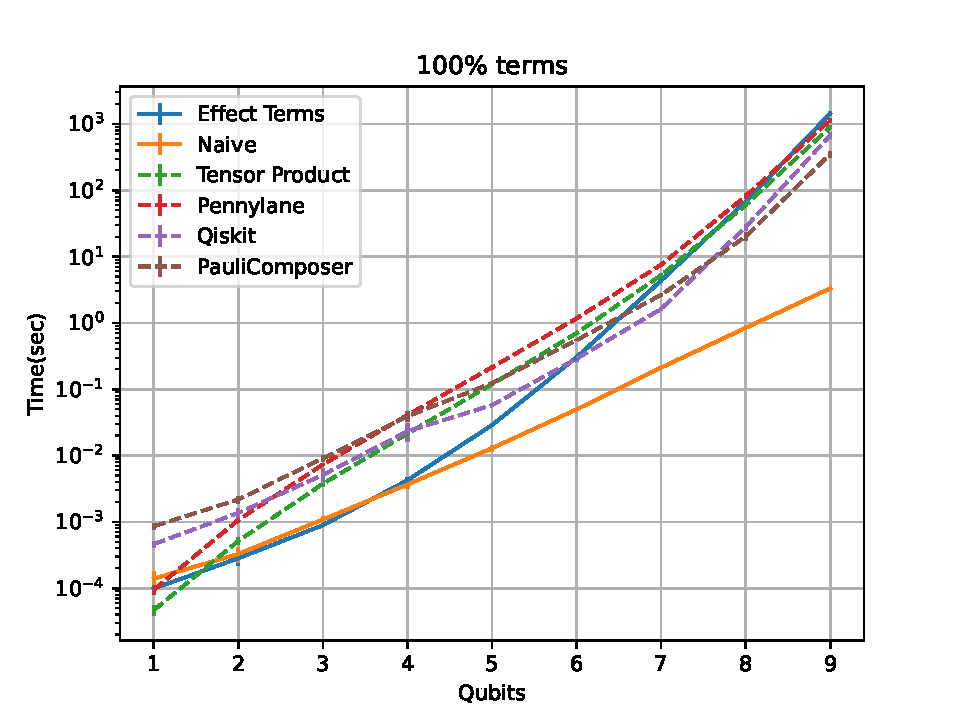
\includegraphics[width=0.7\textwidth]{media/1_terms.pdf}
    \caption{Benchmarks for matrix composition of Puali polynomials with the algorithm 1, 2 with Qiskit, Pennylane,
    PauliComposer, and standard tensor product methods, for $n = 1$ to $n = 9$. The percentages of the each case represents
    how many coefficients are non-empty in $4^n$ number of spaces.}
    \label{fig:composition_benchmark}
\end{figure}